\section{Introduction}
\subsection{Purpose of document}
This report documents the contextualization of a problem surrounding the tracking of truckers.
The background and problem is considered and possible solutions with objectives are identified. 
The scope of the solution and possible benefits are considered.

The research, design and implementation of the postulated solution is documented.
Finally, this solution is evaluated and analyzed, and future recommendations are considered.

\subsection{Background}
Due to the nature of the trucking industry, it is difficult for company owners to keep track of their employees.
Truckers carry out their shifts delivering cargo to various locations over far distances.
As such, it is not possible for employers to track their whereabouts throughout their shifts.

Lack of supervision allows truckers the ability to behave undesirably while on the job.
They can waste time by taking unnecessarily long stops.
Some truckers may drive erratically, unsafely or illegally.
Such employees are a liability to the reputation and profitability of their respective companies.

The ability to track truckers would provide a potential means to address this issue, by allowing employers to monitor their truckers' location, progress and behavior throughout their shifts.
The ability to produce an audit trail detailing the truckers whereabouts during their shifts would allow managers to ensure that work is adequately executed. Such an audit trail would comprise of:
\begin{itemize}
\item \textbf{\ac{gps} coordinates\\}
\ac{gps} tracking will allow employers to ensure that truckers are traveling to required locations, and doing so via effective routes. This also allows employers to ensure no unnecessary detours occur.
\item \textbf{Altitude\\}
Altitude logging may be useful for identifying trends in routes traveled, especially where large altitude gradients occur.
Trucks often struggle traversing steep gradients.
Altitude analysis may offer insight for companies looking to perform optimizations.
\item \textbf{Speed\\}
Examining trucker speeds allows for managers to monitor how quickly truckers are able to transport goods.
Slower routes may be identified where traffic is more prevalent.
This could allow for route optimization, or identifying truck malfunctions.
\item \textbf{Acceleration\\}
Acceleration may be used for inferring any dangerous driving behavior. 
Erratic acceleration and deceleration is associated with dangerous driving.
Additionally, erratic driving can cause more strain and deterioration on the vehicle.
\end{itemize}

The ubiquitous nature of cheap, \ac{gps}-equipped smartphones provides a potential avenue for realizing a simple solution at low cost.
In addition, nation-wide continuous access to the internet allows for live tracking to be utilized most of the time.

\subsection{Problem Statement}
A tracking system must be implemented to be used by trucking companies for tracking and logging their truckers' \ac{gps} coordinates, altitude, speed and acceleration.
Logging data should be collected locally by each trucker using an \ac{iot} device, with network capability.

This data should be continuously (or periodically) made accessible to managers remotely.
To this end, an interface is required for storing, processing and displaying logged data pertaining to the truckers' locations and behavior.
This interface must allow managers to assess the truckers' whereabouts and behavior.

Data presented to truckers must be processed to group log data into separate segments, identifying individual trips.
Any stopping times between must be determined and indicated.

\pagebreak
\subsection{Hypothesis}
A low-cost architecture is proposed in figure \ref{fig:hypothesis}.
This proposal involves the development of a smartphone application capable of interfacing with internal sensors, and transferring sensor data through an \ac{io} server into a data store.
A web interface is postulated for the purposes of displaying processed log data to managers.\cite{bertocco1998client}

\begin{figure}[H]
    \centering
    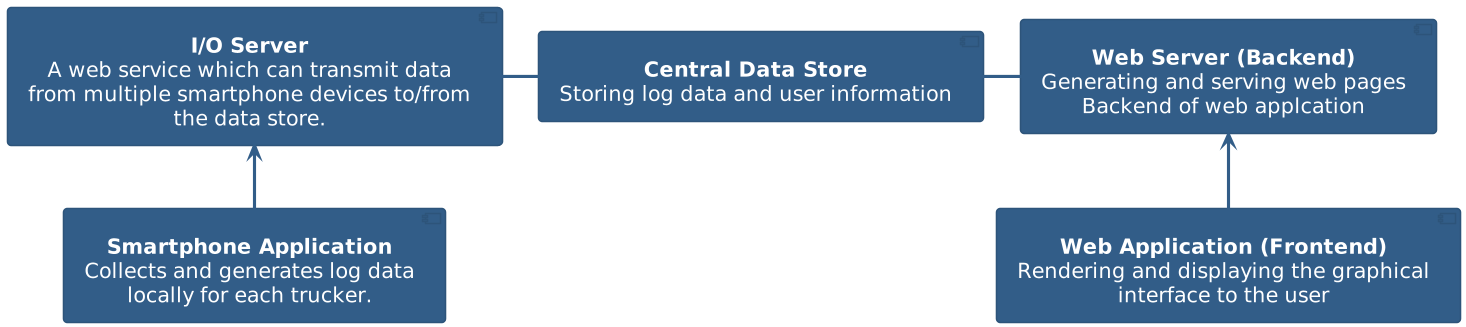
\includegraphics[width=6in]{../diag/hypothesis.png}
    \caption{Proposed high level Architecture}
    \label{fig:hypothesis}
\end{figure}

Smartphones offer great multipurpose capabilities, allowing truckers to communicate and perform other tasks.
They have a rich feature set and have access to a variety of on-board sensors, appealing as a budget-conscious solution.

The \ac{io} server and central data store form part of the necessary infrastructure needed to provide remote capabilities to the system.
The \ac{io} server is a necessary interface to the data store for appropriately handling data capture and ensuring integrity of the log data.
Truckers won't always have stable (peer-to-peer) connections with their managers.
It is therefore necessary to periodically upload and store log data to a central data store, which has high-bandwidth connectivity, allowing easy access for managers.

With web browsers being a ubiquitous component of the modern world, the use of web applications provides easy access, as no extra dependencies are required.
Web servers are needed for handling web application logic and serving the appropriate pages to the manager.
The proposed web application provides managers with data related to their fleet.
This data is extracted from the data store.

\pagebreak
\subsection{Project Objective}
\subsubsection{Primary Objective}
The primary objective in addressing the problem is the development of detailed reports showcasing the truckers' whereabouts and behavior during their work shifts.
These reports must be available to managers for fleet analysis.

\subsection{Anticipated Benefits of Solution}
Managers will be able to ensure that their truckers conduct their work efficiently and responsibly.
They will then be able to adequately handle truckers who fail to perform as expected.
Managers may also be able to analyze trucker behavior to perform fleet optimizations, allowing for increased efficiency.

\subsection{Technical Requirements}
For the realization of the hypothesized solution presented in figure \ref{fig:hypothesis}, the technical requirements and scope definition are defined.

\subsubsection{Requirements}
\begin{enumerate}
\item \textbf{Smartphone Application}\\
    This will be a smartphone application used by the entities being tracked(i.e the truckers).
    \begin{enumerate}
        \item Trucker identification control must be implemented to ensure that logs sent to the server correspond to a unique trucker. It must not be possible for multiple truckers to assume the same or no identity.
        \item Every 2 minutes, sensor data consisting of \textbf{\ac{gps} coordinates, altitude, speed and acceleration} must be captured and stored internally on the smartphone. 
        Data capacity for one continuous week of storage must be possible, to account for connectivity issues.
        \item The application must be able to run in the background, allowing for multitasking.
        \item Sensor data must be uploaded to a central data store, either continuously or on request. This communication must be encrypted for security purposes.
    \end{enumerate}
\item \textbf{\ac{io} Server}\\
This server will facilitate the transfer of logged data from the Smartphone Application to a central data store, via an internet connection. 
    \begin{enumerate}
        \item As a dedicated transfer server, it must exhibit high performance, handling multiple requests from the multiple smartphone clients asynchronously.
        \item Trucker logs, received from smartphone clients, must be stored in a central database.
        \item Information about the trucking company must also be sent to the smartphone client, to confirm the trucker's identity.
    \end{enumerate}

\item \textbf{Data Store}\\
The data store must be efficient, fast and capable of storing large volumes of data.
It should also be capable of adequately interfacing with the \ac{io} server and the web server.

\item \textbf{Web Server and Web Application}\\
The web server must implement backend business logic driving the web application and serving pages to the browser.
The front end of the web application acts as an interface for managers to index truckers and view tracking information about their fleets.
    \begin{enumerate}
        \item Multiple trucking managers must be able to log in and use the application.
        \item Managers must be able to add multiple truckers to their fleet, including trucker-specific information such as name, and vehicle number.
        \item Managers must be able to view detailed trip information for any time period. Log data must be processed to determine starting and arrival times for locations traveled to. Statistical information detailing acceleration, altitude and speed should be displayed, including averages, maximums and percentiles.
    \end{enumerate}
\end{enumerate}
\subsubsection{Scope Definition}
The scope of the problem considered will include
\begin{enumerate}
\item \textbf{Smartphone Application}\\
The defined scope does not include the use of external sensors.
Other measurable variables such as temperature, fuel and pressure are not considered.

The smartphone app is not concerned with displaying user reports and statistics. That is left to the web application.
The smartphone application is purely responsible for logging the appropriate sensor data and transferring this sensor data through the \ac{io} server.
\item \textbf{\ac{io} Server}\\
The \ac{io} server is responsible for facilitating the transfer of sensor data from the smartphone to the data store.
It must implement functionality for handling requests for verifying trucker identity. 
\item \textbf{Data Store}\\
The data store element is purely concerned with the storage of logs, user identity information and providing an interface for the \ac{io} server to query and add records to the store.
Existing data storage systems will be considered.
\end{enumerate}

\subsection{Deliverables}
The proposed deliverables will allow the entire project to function, from the smartphone logging implementation, to detailed reports available in the web application. 
Each deliverable is a standalone component in the proposed solution.
\begin{itemize}
\item Smartphone Application will be created for data logging.
\item \Ac{io} server which will handle requests and query data to the data store.
\item Web Application and web server
\end{itemize}

\subsection{Conclusion}
Basic contextualization of the problem has been performed.
Low level details, however, have not been considered.
Each aspect of the planned architecture may be realized in multiple ways on the low level.
Further research and a feasibility analysis is necessary for adequate low level design.

\pagebreak
